\documentclass[a4paper]{article}

\usepackage[english]{babel}
\usepackage[utf8x]{inputenc}
\usepackage[T1]{fontenc}

\usepackage[a4paper,top=3cm,bottom=2cm,left=3cm,right=3cm,marginparwidth=1.75cm]{geometry}

\usepackage{nth}
\usepackage{amsmath}
\usepackage{graphicx}
\usepackage[hidelinks]{hyperref}
\usepackage{enumitem}

\usepackage{parskip}
\usepackage{lscape}

\newcommand{\ts}{\textsuperscript}
%TODO: Check all paging and add breaks where appropriate.
\title{Integrated Group Project}
\author{NA3
	\\ \rule{5cm}{0.4pt}
	\\Charlie Howes (CH), Lewis Allen (LA), 
    \\Adam Howes (AH), Ben Ashing (BA), 
    \\Constantinos Ioannou (CI)
    \\ \rule{5cm}{0.4pt}
} %TODO: Look at making the rule closer to the text.

\begin{document}
\maketitle

\tableofcontents

\pagebreak

\begin{landscape} %TODO: Look at making this nicer somehow
\section{Planning}
\subsection{Gantt Chart}
\subsubsection{Proposed}
\begin{figure}[!ht] %TODO: Maybe make this landscape, would be easier to read.
    \centering
    \makebox[0.75\textwidth]{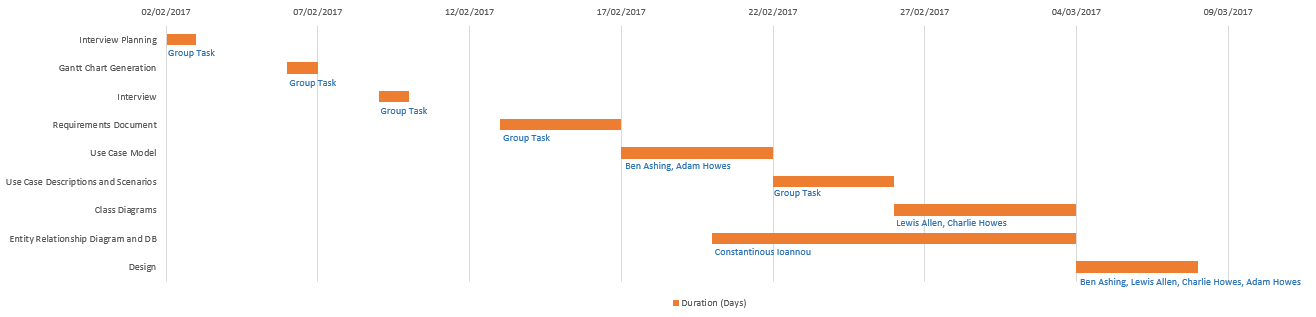
\includegraphics[width=0.75\paperheight]{ProposedGanttChart.png}} %TODO: Check this sizing at the end.
    \caption{Proposed Gantt Chart}
    \label{fig:proposed_gantt}
\end{figure}
\end{landscape}

\subsubsection{Actual} %TODO: This might be better at the end, but not 100% sure.

\subsection{Minutes}

\section{Requirements}

\subsection{Document} %TODO: Need to rename one of these.

\begin{enumerate}
  \item Business Requirements
  \begin{enumerate}[label=B\arabic*.]
    \item The Planning should be completed by March \nth{13}
    \item The finished product should be delivered in May.
    \item The software will be adopted and used by all staff.
  \end{enumerate}

  \item User Requirements
  \begin{enumerate}[label=U\arabic*.] 
    \item Users must be able to log in using a user name and password.
    \item Users must be able to log out
    \item The user must be able to personalize their view.
    \item The user must able to easily view calendars for daily, monthly and yearly schedules.
    \item The user must be able to set recurring appointments.
    \item Staff must be able to create groups.
    \item Staff must be able to modify groups
    \item Staff must be able to add other staff/groups to events.
    \item The user must be able to cancel appointments at any time within a session.
    \item The user must be able to use a search feature to find other users.
    \item The user should be able to make event requests. 
    \begin{enumerate}[label*=\arabic*.]
      \item Users should be able to receive event requests.
      \item Users should be able to accept event requests.
      \item Users should be able to decline event requests.
    \end{enumerate}
  \end{enumerate}

  \item Quality Requirements
  \begin{enumerate}[label=Q\arabic*.]
    \item The application must use symbols to clearly show changes in events.
    \item The application should notify the user in any changes to events such as cancellations.
    \item The application must implement optimized loading times.
  \end{enumerate}
  \item Functional Requirements
  \begin{enumerate}[label=F\arabic*.]
    \item Only members of staff should be assigned accounts.
    \item The architecture of the project should support different platforms.
    \item A method must exist which allows staff to be given administration rights to form an administrative team.
    \item Administrators must be able to verify accounts.
  \end{enumerate}
  \item Non-Functional Requirements
  \begin{enumerate}[label=NF\arabic*.]
  	  \item The user should be able to complete any single task with a minimum of eight actions. (LA)
      \item The code needs to be easily maintainable by keeping the code organized, well written, documented and simple. (CH)
      \item The project must be easily scaled to implement additional features and a larger user base. (CH) %TODO: Be more specific with numbers
      \item The program must be executable on the following Operating Systems: (AH) \begin{itemize}
        \item Windows 8, 8.1 \& 10
        \item Mac OS
        \item Linux Ubuntu
      \end{itemize}
      \item The minimum specifications to run the program should be: (AH) \begin{itemize}
        \item Processor: Pentium 4
        \item RAM: 500MB
        \item Disk Space: 100MB
      \end{itemize}
      \item The code must also be able to run on both 32 and 64-bit Operating Systems and be able to view events when not connected to the Internet. (AH)
      \item All personal data must be fully secure through encryption and hashing. (BA)
      \item The project must be adaptable in the future for mobile implementations. (CI)
  \end{enumerate}
\end{enumerate}

\clearpage % Forces the figure to be in this subsection by clearing the floats.
\subsection{Stakeholder Diagram}

\begin{figure}[!ht]
    \centering
    \makebox[0.75\textwidth]{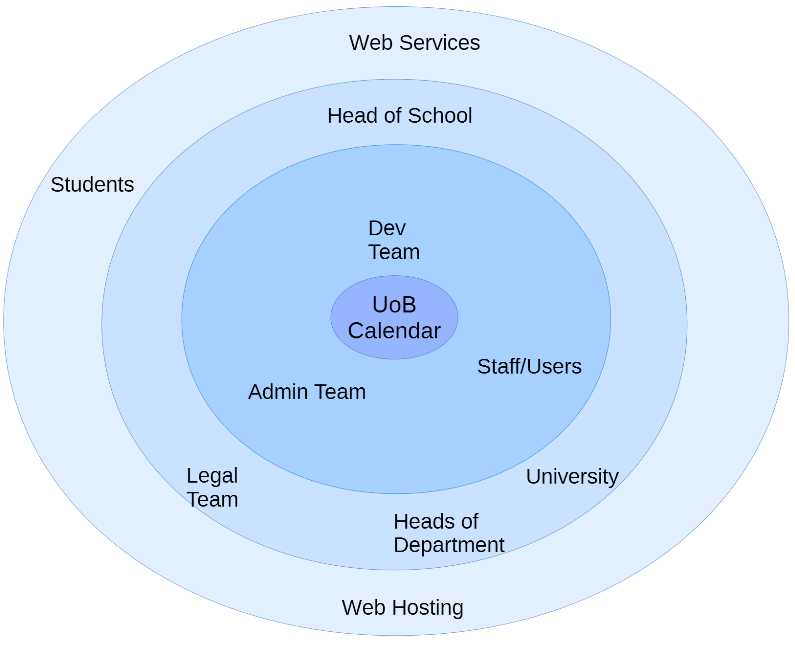
\includegraphics[width=0.75\paperwidth]{OnionModel.png}} %TODO: Check this sizing at the end.
    \caption{Stakeholder Diagram}
    \label{fig:stakeholder}
\end{figure}

\section{Use Case Model}

\subsection{Actors}

\subsection{Diagram}

\subsection{Case Descriptions} %TODO: Add other descriptions when they are done alongside screens.
\subsubsection{Login - CI}
\underline{\textit{Use case}}: Login

\underline{\textit{Actors}}: User (Primary)

\underline{\textit{Goal}}: TODO? %TODO: This was for AeroCar UML Coursework

\underline{\textit{Precondition}}: Time, Date \& Location from customer (via phone).

\underline{\textit{Success postcondition}}: The user fills in their login credentials successfuly and logs into the system.

\underline{\textit{Failure postcondition}}: The user does not fill the correct login credentials.

\underline{\textit{Trigger}}: The personal calendar of the user is displayed

\underline{\textit{Main success scenario}}: 
\begin{enumerate}[leftmargin = 3em]
    \item User wants to login
    \item User inserts credentials into the system
    \item User clicks the login button
    \item System checks the input credentials.
    \item System fetches information and displays their personal calendar
\end{enumerate} 

\underline{\textit{Extensions}}:
\begin{enumerate}[label=3\alph*, leftmargin = 3em]
    \item User entered invalid data \begin{enumerate}[label=\arabic*.]
        \item System asks the user to input correct data
        \item Restart from 2
    \end{enumerate}
\end{enumerate}

\subsubsection{Creating an Event - LA}
\underline{\textit{Use case}}: Creating an Event

\underline{\textit{Actors}}: User (Primary)

\underline{\textit{Goal}}: TODO? %TODO

\underline{\textit{Precondition}}: The User has logged into their account.

\underline{\textit{Success postcondition}}: The User has the created event displayed on their calendar.

\underline{\textit{Failure postcondition}}: The User was unable to create the event.

\underline{\textit{Trigger}}: The User clicks the ‘add event’ button.

\underline{\textit{Main success scenario}}: 
\begin{enumerate}[leftmargin = 3em]
    \item The user clicks the ‘add event’ button.
    \item The User specifies the time, day and duration of the event.
    \item The user names the event and gives it a description.
    \item The user clicks ‘Confirm’.
    \item The System adds the event to the user’s calendar.
\end{enumerate} 

\underline{\textit{Extensions}}:
\begin{enumerate}[label=2\alph*, leftmargin = 3em]
    \item The user has input an event time/date and there is a conflicting schedule. (The user already has an event booked for that duration) \begin{enumerate}[label=\arabic*.]
        \item The System indicates that the user can no longer click confirm.
        \item The System informs the user that there is already an event planned for that duration.
        \item The user is returned to the event creation screen and is given the option to change to event time/day, along with the other details if required.
        \item The user modifies the time/day to a free period.
        \item Continue on to step 3.
    \end{enumerate}
\end{enumerate}

\section{Class Diagram}

\section{Database}
\subsection{Documentation}
\subsubsection{Entities}
\underline{\textit{Event:}} \\
This entity will store all the information about the events. The unique ID for the entity is the \textit{Event\_ID} and it will be used to determine an event. The entity can hold all the necessary information such as date duration and location. The event is created by a user so the \textit{Host\_ID} is used to identify the user that create the event. The option to keep the event private is also available. 

\underline{\textit{Event Request:}} \\
The Event Request entity is used store the information about an event request. The unique ID is the foreign key from the Event entity. It stores the response of user to the request as well as date invited and if the user seen the request or not. 

\underline{\textit{User:}} \\
All the data of a user are store in the User entity. The unique \textit{User\_ID} is used as a primary and is used to log in in to the system with the required password. The basic personal data of the user are also store such as first name, last name, position, email and phone number. An Admin attribute is used to identify if a user is an admin or a normal user. 

\underline{\textit{Attendee:}} \\
The attendee entity holds the information about the attendance of the event. The combination of the two attributes \textit{User\_ID} and \textit{Event\_ID} will give a combine key for the table. 

\subsubsection{Tables}
\begin{table}[ht]
    \caption{Event}
    \centering
    \begin{tabular}{|c|c|c|c|}
        \hline
        Attributes & PK/FK & Data Type & Constraints  \\
        \hline
        Event\_ID & PK & VarChar(10) & Unique, Not Null \\
        \hline
        User\_ID & FK & VarChar(10) & Not Null \\
        \hline
        Host\_ID & & VarChar(10) & Not Null \\
        \hline
        Event\_Description & & VarChar(30) & Not Null \\
        \hline
        Event\_Start\_Date & & Date & Not Null \\
        \hline
        Event\_Duration & & Integer & \\
        \hline
        Room\_No & & VarChar(10) & \\
        \hline
        Location & & VarChar(15) & \\
        \hline
        Private & & Bit & \\
        \hline
        Comment & & VarChar(100) & \\
        \hline
    \end{tabular}
    \label{tab:event}
\end{table}

\begin{table}[ht]
    \caption{Attendee}
    \centering
    \begin{tabular}{|c|c|c|c|}
        \hline
        Attributes & PK/FK & Data Type & Constraints  \\
        \hline
        Event\_ID & FK & VarChar(10) & Unique, Not Null \\
        \hline
        User\_ID & FK & VarChar(10) & Not Null \\
        \hline
    \end{tabular}
    \label{tab:attendee}
\end{table}

\begin{table}[ht]
    \caption{User}
    \centering
    \begin{tabular}{|c|c|c|c|}
        \hline
        Attributes & PK/FK & Data Type & Constraints  \\
        \hline
        User\_ID & PK & VarChar(10) & Unique, Not Null \\
        \hline
        Admin & & Bit & Not Null \\
        \hline
        Password & & VarChar(20) & Not Null \\
        \hline
        First\_Name & & VarChar(15) & Not Null \\
        \hline
        Last\_Name & & VarChar(15) & Not Null \\
        \hline
        Position & & VarChar(30) & \\
        \hline
        Email & & VarChar(30) & \\
        \hline
        Phone\_Number & & VarChar(20) & Not Null \\
        \hline
    \end{tabular}
    \label{tab:user}
\end{table}

\begin{table}[ht] %TODO: Need to fix the vertical positioning of this
    \caption{Event Request}
    \centering
    \begin{tabular}{|c|c|c|c|}
        \hline
        Attributes & PK/FK & Data Type & Constraints  \\
        \hline
        Event\_ID & FK & VarChar(10) & Unique, Not Null \\
        \hline
        Response & & Bit & Not Null \\
        \hline
        Seen & & Bit & Not Null \\
        \hline
        Date\_Invited & & Date & Not Null \\
        \hline
    \end{tabular}
    \label{tab:event_request}
\end{table}

\begin{landscape}
\clearpage
\subsection{Entity Relationship Diagram}
\begin{figure}[!ht] %TODO: Look into making this landscape too
    \centering\makebox[0.9\textwidth]{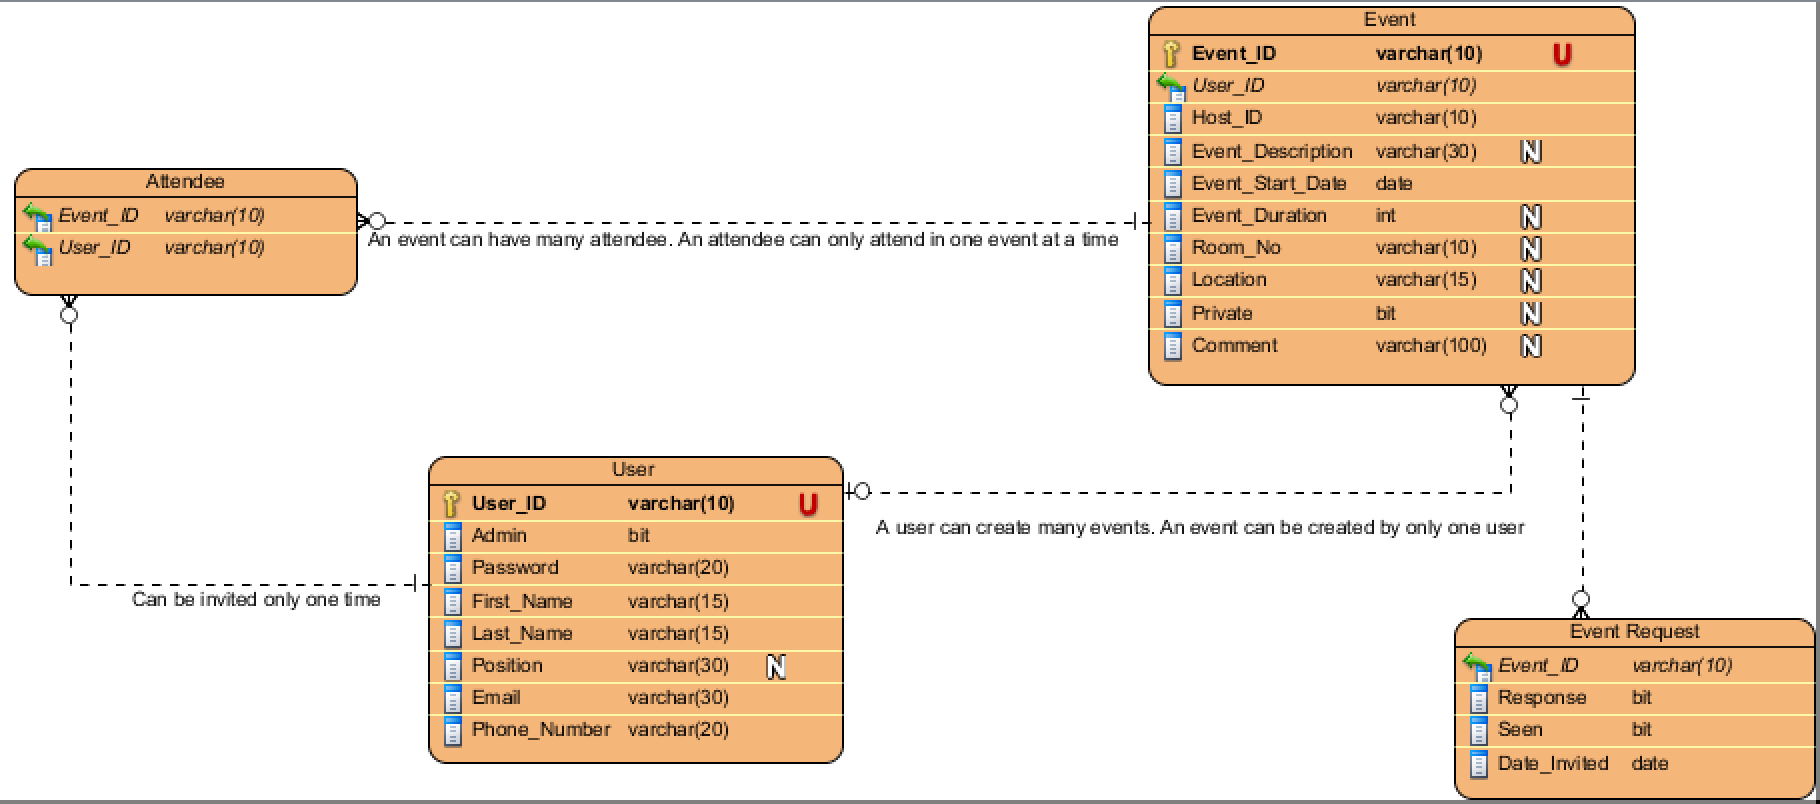
\includegraphics[width=0.75\paperheight]{ERDiagram.png}} %TODO: Check this sizing at the end.
    \caption{Entity Relationship Diagram}
    \label{fig:erd}
\end{figure}
\end{landscape}

\section{Design}

\end{document}